\documentclass[12pt, a4paper, oneside]{ctexart}
\usepackage[margin=2cm]{geometry}%要先设置页边距,否则页眉页脚会偏
\usepackage{amsmath, amsthm, amssymb, bm, graphicx, hyperref, mathrsfs,float,xcolor,color}
\usepackage{listings}

% 用来设置附录中代码的样式

\lstset{
    basicstyle          =   \bf \ttfamily,          % 基本代码风格
    keywordstyle        =   \bfseries,   % 关键字风格
    keywordstyle        =   \color{blue},
    stringstyle         =   \color{magenta},
    commentstyle        =   \color{red}\ttfamily,
    language            =    [x86masm]Assembler,
    commentstyle        =   \rmfamily\itshape,  % 注释的风格,斜体
    escapeinside=``, % 英文分号中可写入中文
    stringstyle         =   \ttfamily,  % 字符串风格
    columns=fullflexible,%可以自动换行
    breaklines=true,%在单词边界处换行。
    numbers             =   left,   % 行号的位置在左边
    showspaces          =   false,  % 是否显示空格,显示了有点乱,所以不现实了
    numberstyle         =   \zihao{-5}\ttfamily,    % 行号的样式,小五号,tt等宽字体
    showstringspaces    =   false,
    captionpos          =   t,      % 这段代码的名字所呈现的位置,t指的是top上面
    frame               =   lrtb,   % 显示边框
}
\title{实验十二 \qquad  演奏乐曲}
\author{学号:61822313 \qquad 姓名:钟锦程 \qquad 实验日期:\today}
\date{}
\begin{document}
\maketitle
\section{实验任务和实验结果}
利用IBM-PC机上的发音装置产生声响与音调,编制音乐演奏程序。
\subsection{基础任务}
\subsubsection{实验任务的具体内容}
根据乐曲“四季歌”的一段简谱,调用SING子程序(其作用是从数据段中取出每个音符的频率数据和节拍时间数据,然后调用SOUND子程序让电脑扬声器发出相应频率和节拍的声音),编制演奏“SONG OF FOUR SEASON”乐曲程序。
在程序的数据段中要定义频率数据(FREQ)和节拍时间数据(TIME),并以0000H作为频率数据结束标志。在代码段中,将频率数据首地址送SI,节拍时间数据的首地址送BP。
\subsubsection{调试通过的源程序}
\begin{lstlisting}
DATA SEGMENT
SONG_NAME DB 'SONG OF FOUR SEASON','$'
SONG_FREQ DW 660 ,660, 588, 524, 588, 524, 494 ;660D=294H 588D=24cH
         DW 440, 440, 440
         DW 698 ,698, 660, 588, 524,588, 698
         DW 660
         DW 698 ,698, 660, 588, 588, 698
         DW 660 ,660 ,524 ,440 ,524
         DW 494 ,660, 588, 524, 494, 524
         DW 440 
         DW 0 
SONG_TIME DW 100, 50, 50, 50, 50, 50, 50
         DW 100, 100, 200
         DW 100, 50, 50, 50, 50, 50 ,50
         DW 400 
         DW 100 ,50 ,50 ,100, 50, 50
         DW 100 ,50 ,50 ,100 ,100
         DW 100 ,100, 50, 50, 50, 50 
         DW 400  
DATA ENDS
STACK SEGMENT
    NN DB 100 DUP(?)
STACK ENDS
CODE SEGMENT 
    ASSUME CS:CODE,DS:DATA,SS:STACK
SING PROC NEAR
    PUSH DI
    PUSH SI
    PUSH BP
    PUSH BX
AGIN: MOV DI,[SI];送频率数据到DI
    CMP DI,0 ;当频率数据不为0,表明还有音符没演奏完
    JE END_SING
    MOV BX,DS:[BP] ;BP默认绑定SS,需要加段前缀.送时间数据
    CALL SOUND ;参数为DI和BX
    ADD SI,2 ;指向下一个频率数据
    ADD BP,2 ;指向下一个时间数据
    JMP AGIN 
END_SING:
    POP BX
    POP BP
    POP SI
    POP DI
    RET
SING ENDP

SOUND PROC NEAR
    PUSH AX
    PUSH BX ;BX节拍时间数据
    PUSH CX
    PUSH DX
    PUSH DI ;入口参数DI给定频率数据
    MOV AL,0B6H ;8253初始化(通道2,方式3,产生方波信号,先送低字节再送高字节)
    OUT 43H,AL ;43H端口是8253的命令寄存器
    MOV DX,0012H ;计算时间常数
    MOV AX,34DCH
    DIV DI ;除法结果在AX中
    OUT 42H,AL ;给8253通道2设置计数初值
    MOV AL,AH
    OUT 42H,AL ;装入计数初值
    IN AL,61H ;读8255B口
    MOV AH,AL
    OR AL,3 ;8255 PB1PB0置1,开喇叭
    OUT 61H,AL
DELAY: 
    MOV CX,15000
DL10ms: 
    LOOP DL10ms ;延时10ms
    DEC BX ;BX=节拍时间对应10ms的倍数,如:BX=100,节拍时间=10ms*100=1s
    JNZ DELAY
    MOV AL,AH
    OUT 61H,AL ;8255 PB1PB0恢复为零,关喇叭
DL20MS:
    LOOP DL20MS;Z这一行让每个音符单独发声不连音
    MOV AL,AH
    ;OUT 61H,AL ;8255 PB1PB0恢复为零,关喇叭
    POP DI
    POP DX
    POP CX
    POP BX
    POP AX
    RET
SOUND ENDP
START:
    MOV AX,DATA 
    MOV DS,AX 
    MOV AX,STACK
    MOV SS,AX
    MOV ax,OFFSET SONG_NAME
    mov dx,ax
    MOV AH,9
    INT 21H  
    MOV SI,OFFSET SONG_FREQ 
    MOV BP,OFFSET SONG_TIME 
    CALL SING 
    MOV AH,4CH 
    INT 21H 
CODE ENDS
END START 
\end{lstlisting}
\subsubsection{程序解释}
数据段中SONG-FREQ和SONG-TIME事先存放简谱中各音符的频率和时值,主程序先调用DOS功能,显示歌名。然后调用SING程序,不断按次序读取频率和时值,并调用SOUND子程序发声。程序一直读到频率为零才退出
\subsubsection{实验结果}
如图\ref{基础实验结果截图1}是程序运行的截图,显示"SONG OF FOUR SEASON"之后,程序自动演奏乐曲,演奏结束后返回DOS,如图\ref{基础实验结果截图2}。
\begin{figure}[H]
    \centering
    \begin{minipage}{0.45\textwidth}
    \centering
    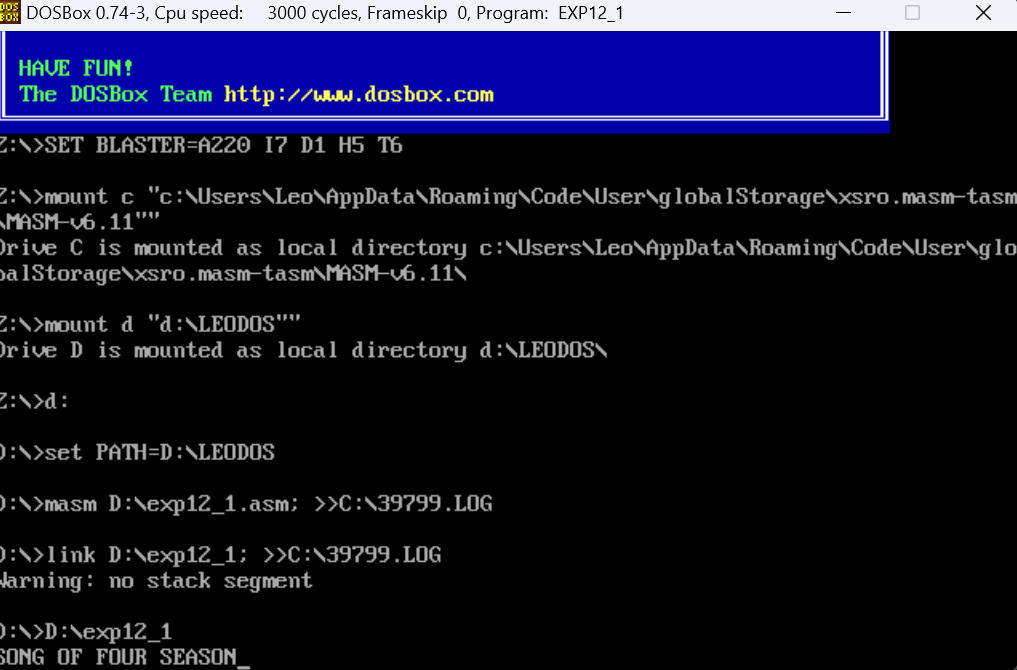
\includegraphics[scale=0.40]{pic/exp12-1.png}
    \caption{基础实验任务结果截图1}
    \label{基础实验结果截图1}
    \end{minipage}
    \hspace{0.05\textwidth}
    \begin{minipage}{0.45\textwidth}
    \centering
    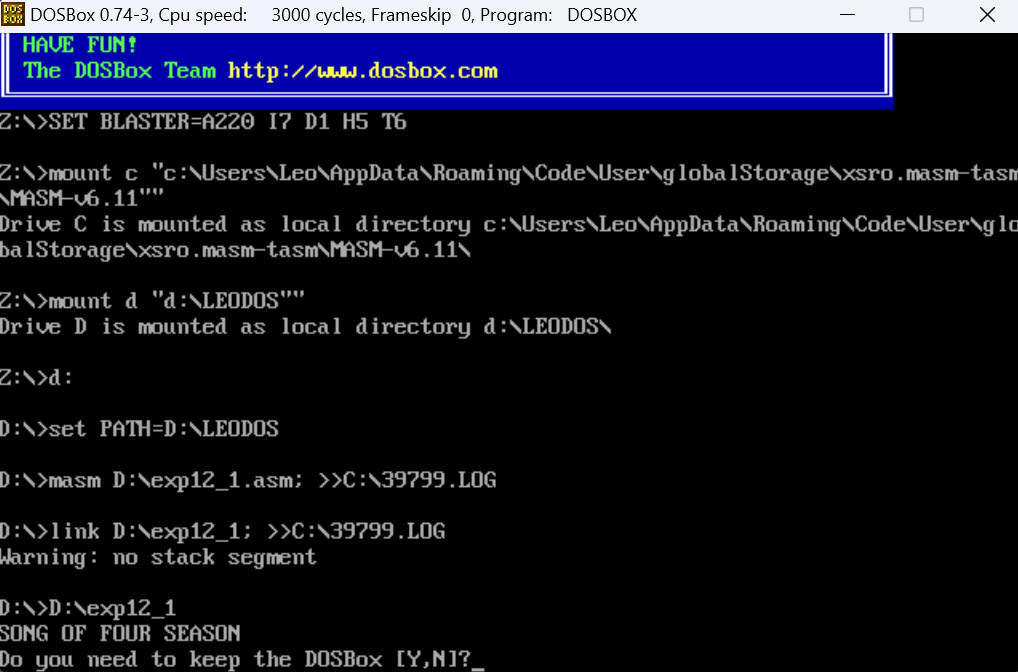
\includegraphics[scale=0.40]{pic/exp12-1-1.png}
    \caption{基础实验任务结果截图2}
    \label{基础实验结果截图2}
    \end{minipage}
\end{figure}
\subsection{附加任务1:演奏有休止符的另一首乐曲}
\subsubsection{实验任务的具体内容}
提供乐谱,解释程序中频率和节拍数据与乐谱之间的对应关系。(要求在演奏的乐曲中加入休止符)
\subsubsection{调试通过的源程序}
\begin{lstlisting}
DATA SEGMENT
SONG_NAME DB 'JINGO BELL','$'
SONG_FREQ DW 330,330,330
DW 330,330,330
DW 330,392,262,294
DW 330,0F000H;44个
DW 349,349,349,349
DW 349,330,330,330,330
DW 330,294,294,262
DW 294,392,0F000H

DW 330,330,330
DW 330,330,330
DW 330,392,262,294
DW 330,0F000H;44个
DW 349,349,349,349
DW 349,330,330,330,330
DW 392,392,440,494
DW 524,0F000H
DW 0
SONG_TIME DW 50,50,100
DW 50,50,100
DW 50,50,75,25
DW 100,100
DW 50,50,75,25
DW 50,50,50,25,25
DW 50,50,50,50
DW 100,50,60

DW 50,50,100
DW 50,50,100
DW 50,50,75,25
DW 100,100
DW 50,50,75,25
DW 50,50,50,25,25
DW 50,50,50,50
DW 100,100
DATA ENDS
STACK SEGMENT
    NN DB 100 DUP(?)
STACK ENDS
CODE SEGMENT 
    ASSUME CS:CODE,DS:DATA,SS:STACK
SING PROC NEAR
    PUSH DI
    PUSH SI
    PUSH BP
    PUSH BX
AGIN: MOV DI,[SI];送频率数据到DI
    CMP DI,0 ;当频率数据不为0,表明还有音符没演奏完
    JE END_SING
    MOV BX,DS:[BP] ;BP默认绑定SS,需要加段前缀.送时间数据
    CALL SOUND ;参数为DI和BX
    ADD SI,2 ;指向下一个频率数据
    ADD BP,2 ;指向下一个时间数据
    JMP AGIN 
END_SING:
    POP BX
    POP BP
    POP SI
    POP DI
    RET
SING ENDP

SOUND PROC NEAR
    PUSH AX
    PUSH BX ;BX节拍时间数据
    PUSH CX
    PUSH DX
    PUSH DI ;入口参数DI给定频率数据
    MOV AL,0B6H ;8253初始化(通道2,方式3,产生方波信号,先送低字节再送高字节)
    OUT 43H,AL ;43H端口是8253的命令寄存器
    MOV DX,0012H ;计算时间常数
    MOV AX,34DCH
    DIV DI ;除法结果在AX中
    OUT 42H,AL ;给8253通道2设置计数初值
    MOV AL,AH
    OUT 42H,AL ;装入计数初值
    IN AL,61H ;读8255B口
    MOV AH,AL
    OR AL,3 ;8255 PB1PB0置1,开喇叭
    OUT 61H,AL
DELAY: 
    MOV CX,15000
DL10ms: 
    LOOP DL10ms ;延时10ms
    DEC BX ;BX=节拍时间对应10ms的倍数,如:BX=100,节拍时间=10ms*100=1s
    JNZ DELAY
    MOV AL,AH
    OUT 61H,AL ;8255 PB1PB0恢复为零,关喇叭
DL20MS:
    LOOP DL20MS;Z这一行让每个音符单独发声不连音
    MOV AL,AH
    OUT 61H,AL ;8255 PB1PB0恢复为零,关喇叭
    POP DI
    POP DX
    POP CX
    POP BX
    POP AX
    RET
SOUND ENDP

START:
    MOV AX,DATA 
    MOV DS,AX 
    MOV AX,STACK
    MOV SS,AX
    MOV ax,OFFSET SONG_NAME
    MOV DX,AX
    MOV AH,9
    INT 21H  
    MOV SI,OFFSET SONG_FREQ 
    MOV BP,OFFSET SONG_TIME 
    CALL SING 
    MOV AH,4CH 
    INT 21H 
CODE ENDS
END START 
\end{lstlisting}
\subsubsection{程序解释}
电脑中,8253的计数时钟频率为1193180Hz,对应发生频率的计数值可按下式计算:1193180/f=1234DCH/f。对于音符的时值控制,节拍数BX=节拍时间对应10ms的倍数,如:BX=100,节拍时间=10ms*100=1s。预先规定1拍对应BX=100,每个小节BX之和应该等于400.在数据段事先装入《铃儿响叮当》的简谱对应的频率和时值数据。主程序调用SING,SING调用SOUND的基本逻辑不变。改变之处在于:
\begin{enumerate}
    \item 加入休止符。实现方法为:在需要插入休止符的地方放置一个相同时长的超高频率,这样在演奏时由于超出人耳接收范围而听起来像没有声音
    \item 能够分辨同音调连音:这首歌的同音调连音很多,如果不修改SOUND程序,声音会连成一片效果不好。为解决此问题,在SOUND子程序中关喇叭后延时一小段时间,使相邻音符之间有间隙。
\end{enumerate}
\subsubsection{实验结果}
如图\ref{附加任务1结果截图1}是所演奏的简谱(0即为休止符)。图\ref{附加任务1结果截图2}是演奏开始时显示乐曲名的截图。
\begin{figure}[H]
    \centering
    \begin{minipage}{0.45\textwidth}
    \centering
    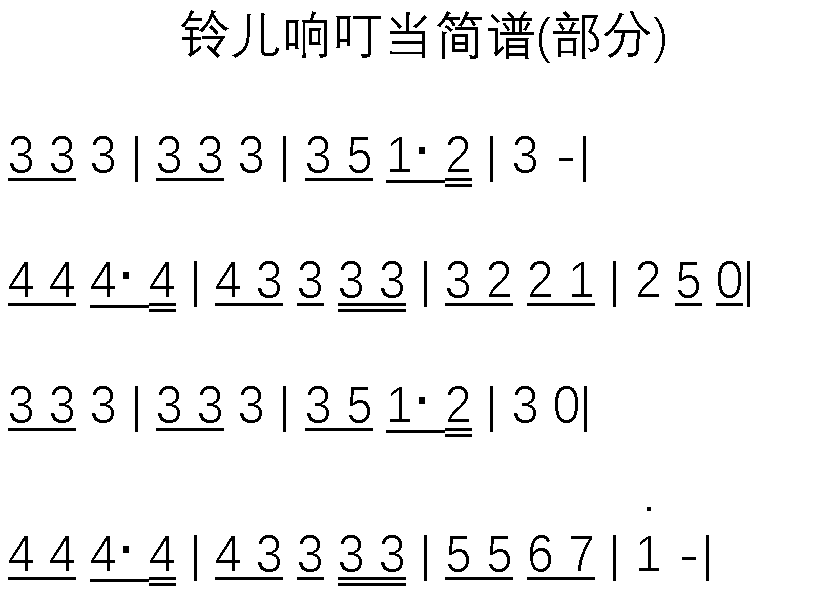
\includegraphics[scale=0.45]{pic/简谱.png}
    \caption{附加任务1结果截图1}
    \label{附加任务1结果截图1}
    \end{minipage}
    \hspace{0.05\textwidth}
    \begin{minipage}{0.45\textwidth}
    \centering
    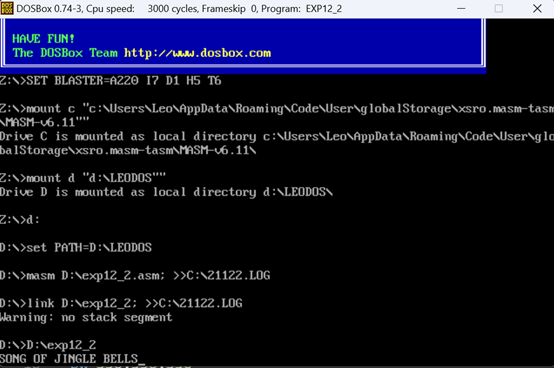
\includegraphics[scale=0.50]{pic/exp12-2-1.png}
    \caption{附加任务1结果截图2}
    \label{附加任务1结果截图2}
    \end{minipage}
\end{figure}
\subsection{附加任务2:用键盘模拟电子琴}
\subsubsection{实验任务的具体内容}
用键盘模拟电子琴演奏乐曲;
1.显示一些提示信息;

比如:高音/中音/低音的7个音和键盘按键字符的对应关系,按什么键结束演奏等;

2.至少能模拟中音的7个音,最好高、中、低音都能模拟;

3.弹奏时,发声可以固定时长(如1秒、2秒…),最好能模拟电子琴真实的发声,键按下发声,键松开不发声。
\subsubsection{调试通过的源程序}
\begin{lstlisting}
DATA SEGMENT 
    KEY2ASCII DB 'THE KEY TABLE:',0DH,0AH
              DB 'Q:1^ W:2^ E:3^ R:4^ T:5^ Y:6^ U:7^',0DH,0AH
              DB 'A:1 S:2 D:3 F:4 G:5 H:6 J:7',0DH,0AH
              DB 'Z:1_ X:2_ C:3_ V:4_ B:5_ N:6_ M:7_',0DH,0AH 
              DB 'PRESS P TO QUIT',0DH,0AH,'$'
    KEY2FREQ DW 524, 588, 660, 698, 784, 880, 988
                DW 262, 294, 330, 349, 392, 440, 494
              DW 131, 147, 165, 175, 196, 220, 247 
    QUIT_FLAG DB 0;=1时应该退出,返回dos
DATA ENDS 
STACK SEGMENT
    NN DB 100 DUP(?)
STACK ENDS
CODE SEGMENT 
    ASSUME CS:CODE,DS:DATA
KEYINT PROC FAR 
    PUSH AX
    PUSH BX 
    PUSH DX 
    STI 
    IN AL,60H      ; 通过8255A的PA口(PA口地址为60H)读取键盘扫描码
    MOV AH,AL
    IN AL,61H      ; 从8255APB口(PB口地址为61H)的PB7输出一个正脉冲(即PB7先输出高电平,再输出低电平)
    OR AL,80H      ; PB7置1
    OUT 61H,AL
    AND AL,7FH     ; PB7清零,表示可以接收下一次键盘中断
    OUT 61H,AL     
    TEST AH,80H    ; AH中是最开始的键盘扫描码。不相等时表示键被按下,应该开喇叭并发出对应的声音;相等时代表键被释放,应该关喇叭
    JE SOUND_ON
    JMP SOUND_OFF   
SOUND_OFF:
    MOV AL,0
    CMP AH,90H  
    JAE HIGH_KEY2 ;>90H,进入有效键范围的下界
    JMP BACK1 ;低于90h的不在有效键范围内
HIGH_KEY2:
    CMP AH,9EH 
    JAE MID_KEY2 ;>9EH的跳转,小于的说明是q-u,高音区
    CMP AH,96H 
    JA BACK1 ;>96H,无效键
    JMP CLOSE_HORN
MID_KEY2:
    CMP AH,0ACH
    JAE LOW_KEY2 ;>0ACH的跳转,小于的留下,说明是a-j,中音区
    CMP AH,0A4H 
    JA BACK1 ;>0A4H,无效键
    JMP CLOSE_HORN
LOW_KEY2:
    CMP AH,0B2H
    JA BACK1 ;>0B2H的跳转结束,小于的说明是z-m,低音区
    JMP CLOSE_HORN
CLOSE_HORN:
    IN AL,61H ;读8255B口
    AND AL,11111100B ;8255 PB1PB0置0,关喇叭
    OUT 61H,AL
    JMP BACK1
BACK1:
    JMP BACK
SOUND_ON:
    CMP AH,19H ;p 按下19松开99
    JNE GO
    MOV AH,1 
    MOV QUIT_FLAG,AH ;打上退出标记,使得返回主程序时可以退出到dos
    JMP BACK 
GO:
    MOV AL,00H
    CMP AH,10H  
    JAE HIGH_KEY ;>10,进入有效键范围的下界
    JMP BACK ;低于10h的不在有效键范围内
HIGH_KEY:
    CMP AH,1EH 
    JAE MID_KEY ;>1EH的跳转,小于的说明是q-u,高音区
    CMP AH,16H 
    JA BACK ;>16H,无效键
    AND AH,0FH ;取AH低4位,正好可以作为位移量
    JMP OPEN_HORN
MID_KEY:
    CMP AH,2CH
    JAE LOW_KEY ;>2CH的跳转,小于的留下,说明是a-j,中音区
    CMP AH,24H 
    JA BACK ;>24H,无效键
    SUB AH,23 ;取AH-23,正好可以作为位移量
    JMP OPEN_HORN 
LOW_KEY:
    CMP AH,32H
    JA BACK
    SUB AH,30 ;取AH-30,正好可以作为位移量
    JMP OPEN_HORN
OPEN_HORN:
    MOV AL,0
    XCHG AL,AH
    MOV DL,2
    MUL DL
    MOV BX,AX
    MOV DI,DS:[SI+BX] ;送频率数据(之前要保证SI指向频率数据首址 )
    CALL SOUND_UP
    JMP BACK
BACK:
    STI   
    MOV AL,20H
    OUT 20H,AL;结束中断
    POP DX
    POP BX
    POP AX
    IRET 
KEYINT ENDP 

SOUND_UP PROC NEAR
    PUSH AX
    PUSH BX 
    PUSH CX
    PUSH DX
    PUSH DI ;入口参数DI给定频率数据
    MOV AL,0B6H ;8253初始化(通道2,方式3,产生方波信号,先送低字节再送高字节)
    OUT 43H,AL ;43H端口是8253的命令寄存器
    MOV DX,0012H ;计算时间常数
    MOV AX,34DCH
    DIV DI ;除法结果在AX中
    OUT 42H,AL ;给8253通道2设置计数初值
    MOV AL,AH
    OUT 42H,AL ;装入计数初值
    IN AL,61H ;读8255B口
    MOV AH,AL
    OR AL,3 ;8255 PB1PB0置1,开喇叭
    OUT 61H,AL
    POP DI
    POP DX
    POP CX
    POP BX
    POP AX
    RET
SOUND_UP ENDP
DELAY PROC         ; 延时程序
    PUSH CX
    PUSH DX
    MOV DX,16H
DL500:
    MOV CX, 0FFFFH
DL10MS:
    LOOP DL10MS
    DEC DX
    JNZ DL500
    POP DX
    POP CX    
    RET
DELAY ENDP
START:
    MOV AX,DATA 
    MOV DS,AX 
    MOV AX,STACK
    MOV SS,AX
    MOV AX,0
    MOV ES,AX
    MOV AH,35H ;INT 21H 35H号:取中断向量,入口AL=中断类型,出口ES:BX=中断向量
    MOV AL,9
    INT 21H 
    PUSH BX ;将原键盘中断处理程序的CS:IP压栈
    PUSH ES 
    MOV AX,0 ;恢复ES!重要!
    MOV ES,AX
    PUSH DS ;保护DS与DX!重要!
    PUSH DX
    CLI
    MOV AX,SEG KEYINT ;将自定义键盘中断服务程序的地址放入原09号中断向量处
    MOV DS,AX
    MOV DX,OFFSET KEYINT
    MOV AL,9
    MOV AH,25H ;INT 21H 25H号:设置中断向量,入口DS:DX=中断向量,AL=中断类型号
    INT 21H
    STI
    POP DX 
    POP DS   
    MOV DX,OFFSET KEY2ASCII ;显示键盘信息
    MOV AH,09H
    INT 21H
    MOV SI,OFFSET KEY2FREQ
    STI
AGIN:
    CALL DELAY
    MOV BL,QUIT_FLAG
    CMP BL,1
    JNE AGIN
    POP DS ;恢复原键盘中断的中断向量
    POP DX
    MOV AL,9
    MOV AH,25H
    INT 21H
    MOV AH,4CH
    INT 21H
CODE ENDS
    END START
\end{lstlisting}
\subsubsection{程序解释}
在数据段装入提示信息,程序启动后显示,高音区为Q-U,中音区为A-J,低音区为Z-M,通过按P键退出程序返回DOS。程序基本思路:主程序循环调用延时程序,并在每次循环中检查退出标志QUIT-FLAG,若不为1则继续循环。重写键盘中断程序:键盘上每一个键按下时会通过键盘中断送来8bit键盘扫描码X,松开某键时也会送来8bit键盘扫描码Y。通过查键盘扫描码表,编写一个略显复杂的比较逻辑,就可以判断出按的是哪一个音区的键,再分析不同音区中按键的扫描码,对其做一些处理,就可以将21个键编码到0-20的区间里。比如高音区的键盘扫描码可以通过取低四位得到0-6,正好作为频率数据块的偏移量。用此偏移量去取得频率值,再调用SOUND-UP子程序打开喇叭实现发声。当按键松开时同理,只不过判断出音区后直接跳转到CLOSE-HORN关喇叭即可,不用再把键扫描码编码到0-20的区间里。特别地,判断某次按键的码是否是P的扫描码(19H),若是,将数据区的QUIT-FLAG置为一,这样当本次中断返回后,主程序检查QUIT-FLAG,可以退出到DOS。
\subsubsection{实验结果}
如图\ref{附加任务2结果截图1}是程序刚开始运行的截图,显示了21个音符对应的按键以及退出按键。之后用户可以根据提示按键发声,结束后按P返回DOS,如图\ref{附加任务2结果截图2}所示。
\begin{figure}[H]
    \centering
    \begin{minipage}{0.45\textwidth}
    \centering
    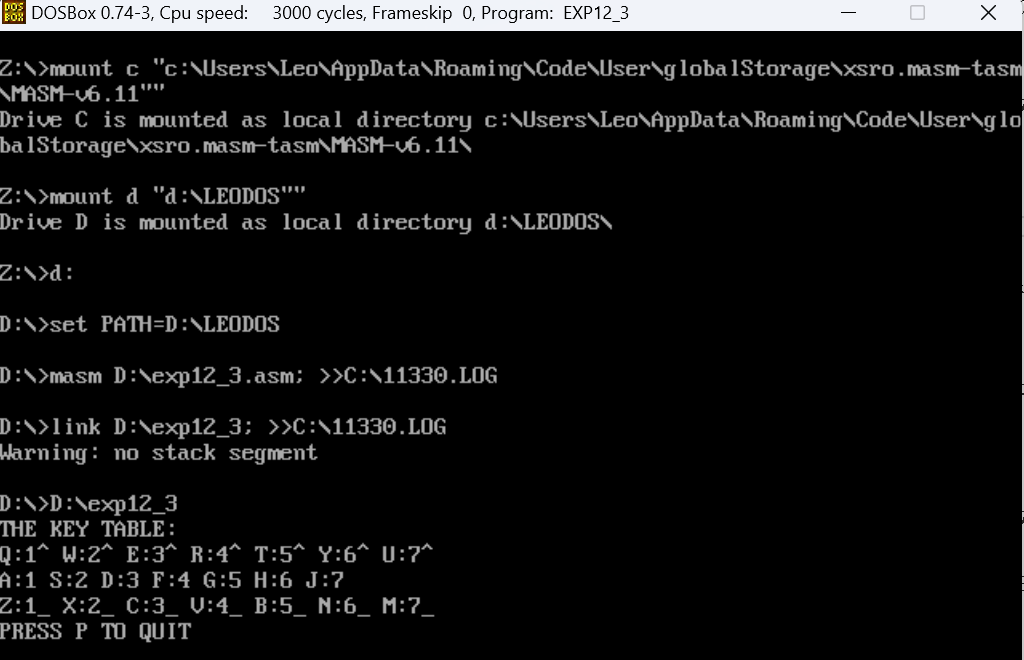
\includegraphics[scale=0.40]{pic/exp12-3-1.png}
    \caption{附加任务2结果截图1}
    \label{附加任务2结果截图1}
    \end{minipage}
    \hspace{0.05\textwidth}
    \begin{minipage}{0.45\textwidth}
    \centering
    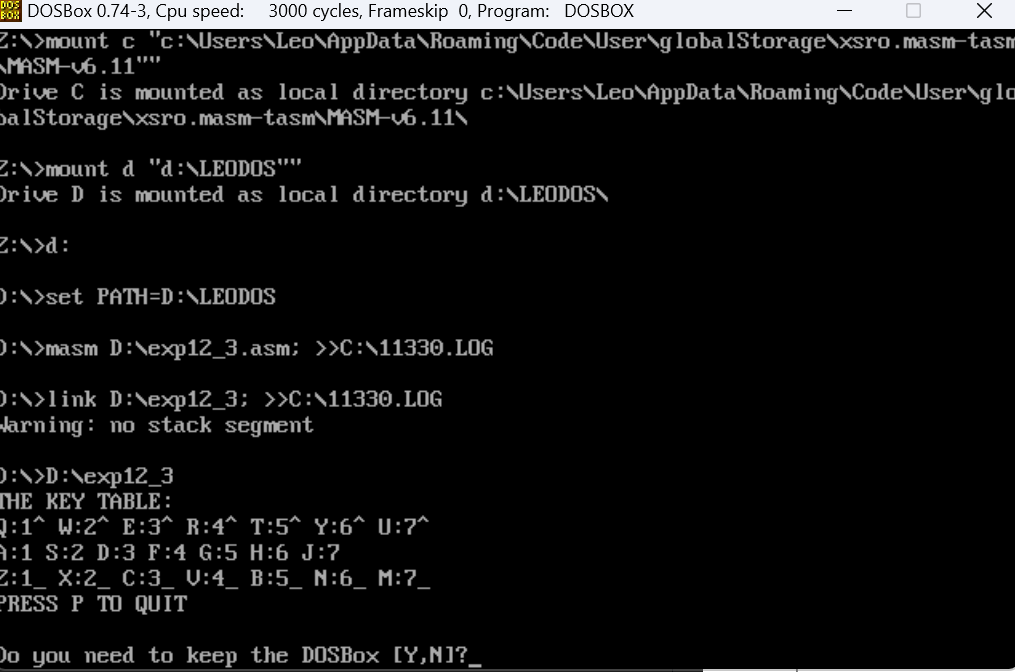
\includegraphics[scale=0.40]{pic/exp12-3-2.png}
    \caption{附加任务2结果截图2}
    \label{附加任务2结果截图2}
    \end{minipage}
\end{figure}
\section{实验总结}
\subsection{基础任务中遇到的问题及解决办法}
\begin{enumerate}
    \item 最开始程序一直显示乱码,后来发现是由于频率区的数字之间加的是空格而不是逗号。
    \item 将歌名所在区域命名为TITLE会发生未知错误,推测可能是由于保留字被占用,更换区域名为SONG-NAME后解决。
\end{enumerate}
\subsection{附加任务1中遇到的问题及解决办法}
\begin{enumerate}
    \item 同音调音符之间连音,演奏效果不好,为此,在每次发声后添加一个适当长的延时,做到音符之间间隔明显。
\end{enumerate}
\subsection{附加任务2中遇到的问题及解决办法}
\begin{enumerate}
    \item 没有把键盘按键与音符的对应关系写到主程序中,而是重写了键盘中断程序,导致调试困难(TD不方便跳转进中断处理程序查看)。解决办法:在需要监视的地方通过DOS功能调用显示一些提示字符辅助调试。调试成功后删掉这些部分。
    \item 高音区对应的扫描码数值低于低音区的扫描码,最开始忽略了这一点导致音调对应错误。
    \item 没有用一一对应的方法将扫描码转换为频率值,而是用一些比较复杂的判断逻辑来实现扫描码到频率值的转换。通过上面所述的调试方法,发现所有按键松开时都会进入退出子程序。解决办法:重写判断逻辑,并把对退出键的判断提到最前面。
    \item 松开按键无法正常退出中断子程序。解决该异常时,发现这样一个现象:按下按键时,程序能正常运行正常退出中断,但松开按键时却出现异常(具体表现为一直显示退出中断的提示字,但该子程序并没有涉及到任何循环)。然而按下和松开用的是同一段代码(BACK)。进一步分析发现松开按钮所在的程序和BACK相隔较远,由此联想到可能因为程序段间距过大跳转出错。解决办法:让松开按键时先进入一个较近的BACK1,再从BACK1跳转到BACK。
    \item 键盘扫描码存在AH中,变换后要拿去加到SI(此时SI已经指到频率区首址)上才能指到频率数据。但是最开始没有交换AL与AH就直接把AX与SI相加,导致频率数据取错,音调错乱。
\end{enumerate}
\section{思考题}
% 1.若要求乐曲中有休止符,程序中应如何实现?
% 2.如果要用键盘模拟电子琴演奏乐曲,请说明程序设计思路。
% 3. 如果完成了附加任务1,请举例解释一下程序中频率数据(以及8253计数通道2的计数初值计算)、节拍数据与乐谱之间的对应关系。
\begin{enumerate}
    \item 在需要加休止符的地方放一个超过人耳接收范围的频率(如本程序用的是0F000H=614\\40Hz),其时值等于需要休止的时值.
    \item 主程序循环调用延时程序,并在每次循环中检查退出标志 QUIT-FLAG,若不为 1 则继续循环。重写键盘中断程序:键盘上每一个键按下时会通过键盘中断送来 8bit 键盘扫描码 X,松开某键时也会送来 8bit 键盘扫描码 Y。通过查键盘扫描码表,判断扫描码所在范围就可以知道按的是哪一个音区的键,再分析不同音区中按键的扫描码,对其做一些处理,就可以将 21 个键编码到 0-20 的区间里。比如高音区的键盘扫描码可以通过取低四位得到 0-6,正好作为频率数据块的偏移量。用此偏移量去取得频率值,再调用 SOUND-UP 子程序打开喇叭实现发声。当按键松开时同理,只不过判断出音区后直接跳转到 CLOSE-HORN 关喇叭即可。
    \item 如附加任务1中演奏的前三个音,其频率数据为330Hz。电脑中,8253的计数时钟频率为1193180Hz,1193180/330=3616.8253 定时/计数通道2调到方波发生器工作方式,并将3616写入计数初值。该计数方式下,每计数到3616的一半会反转一次电平,形成方波。该方波的周期为$\frac{1}{1193180}\times 3616=3.030557\times 10^{-3}s$,频率为$\frac{1}{3.030557\times 10^{-3}}=329\approx330Hz$,将这个方波信号输出到扬声器就可以得到频率为330Hz的声音,对应中音区的"mi".
\end{enumerate}

\end{document}